\section{Regression and Optimization \pts{18}}

\begin{questions}

\question[1] \textbf{True or False:} In order to perform gradient descent, we need to be able to evaluate the objective function.
    \begin{checkboxes}
        \choice True 
        \choice False
    \end{checkboxes}
    \begin{soln}
       False
    \end{soln}
    \begin{qauthor}
        Henry
    \end{qauthor}

\question[1] Suppose that instead of being able to compute the gradient of an objective function for ourselves, the only way we can access the gradient is through a black-box oracle, i.e., some function that takes a setting of the parameters and returns the gradient of the objective function at that location. 
\\
\\
\textbf{True or False:} We can still implement gradient descent in this setting. 
    \begin{checkboxes}
        \choice True 
        \choice False
    \end{checkboxes}
    \begin{soln}
       True
    \end{soln}
    \begin{qauthor}
        Henry
    \end{qauthor}

\begin{EnvFullwidth}

A function $f\colon \mathbb{R}^M \to \mathbb{R}$ is said to be \emph{concave} if $\forall$ $\vec{x}, \vec{x}' \in \mathbb{R}^M$ and $t \in [0,1]$ 
\[
    f\big(t\vec{x}+(1-t)\vec{x}'\big) \ge tf(\vec{x})+(1-t)f(\vec{x}').
\]
Similarly, a function is said to be \emph{strictly concave} if $\forall$ $\vec{x}, \vec{x}' \in \mathbb{R}^M$ (where $\vec{x} \ne \vec{x}'$ ) and $t \in (0,1)$ 
\[
    f\big(t\vec{x}+(1-t)\vec{x}'\big) > tf(\vec{x})+(1-t)f(\vec{x}').
\]
Another convenient definition is that a function $f$ is concave if its second derivative is always $\le 0$ and is strictly concave if its second derivative is always $< 0$. % (\textbf{AUTHOR'S NOTE:} is this hint necessary?)

\end{EnvFullwidth}

\question[1] \textbf{True or False:} $f(x) = ax+b$ is strictly concave over the domain $x \in (-\infty, \infty)$ $\forall$ $a, b \in \mathbb{R}$
    \begin{checkboxes}
        \choice True 
        \choice False
    \end{checkboxes}
    \begin{soln}
       False
    \end{soln}
    \begin{qauthor}
        Henry
    \end{qauthor}
    
\question[1] \textbf{True or False:} $f(x) = \textrm{log}(x)$ is strictly concave over the domain $ x\in (0,\infty)$
    \begin{checkboxes}
        \choice True 
        \choice False
    \end{checkboxes}
    \begin{soln}
       True
    \end{soln}
    \begin{qauthor}
        Henry
    \end{qauthor}


\question[1] Gradient \emph{ascent} is where we repeatedly take steps in the direction of the gradient as opposed to in the direction of the negative gradient.
\\
\\
\textbf{True or False:} Gradient ascent can be used to find the unique global maximum of a strictly concave function.
    \begin{checkboxes}
        \choice True 
        \choice False
    \end{checkboxes}
    \begin{soln}
       True
    \end{soln}
    \begin{qauthor}
        Henry
    \end{qauthor}  
    
\clearpage

\question Suppose you have a regression dataset with one input feature, $x$, and one output value $y$. You wish to evaluate various regression techniques.

\begin{parts}

\part[2] Draw the function that a linear regression model would learn on the dataset below.

    \begin{center}
    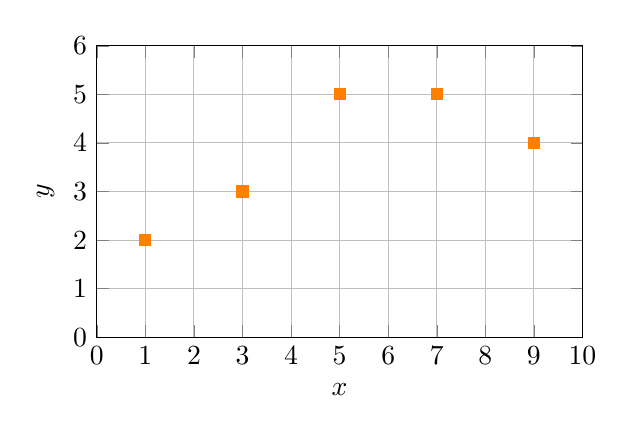
\begin{tikzpicture}
    \begin{axis}[
        scale=0.9, axis equal image,
        xmin=0, xmax=10, xtick={0,...,10},
        ymin=0, ymax=6, ytick={0,...,6},
        samples=50, grid=major, xlabel=$x$, ylabel=$y$]
        \addplot [
            scatter,
            only marks,
            point meta=explicit symbolic,
            scatter/classes={
                a={mark=square*,orange},
                b={mark=triangle*,red}
            },
            nodes near coords*={},
            visualization depends on={\thisrow{myvalue} \as \myvalue},
        ] table [meta=label] {
            x y label myvalue
            1 2 a 1
            3 3 a 1
            5 5 a 1
            7 5 a 1
            9 4 a 1
        };
    \end{axis}
    \end{tikzpicture}
    \end{center}
    \begin{soln} Any straight line that roughly passes through the points should get full credit; a pretty reasonable choice is the line that connects the first, second and fourth points from the left. \end{soln}
    \begin{qauthor} Matt (Solution by Henry) \end{qauthor}

\part[2] Draw the function that a $k$-nearest neighbor regression model with $k=1$ would learn on the dataset below.

    \begin{center}
    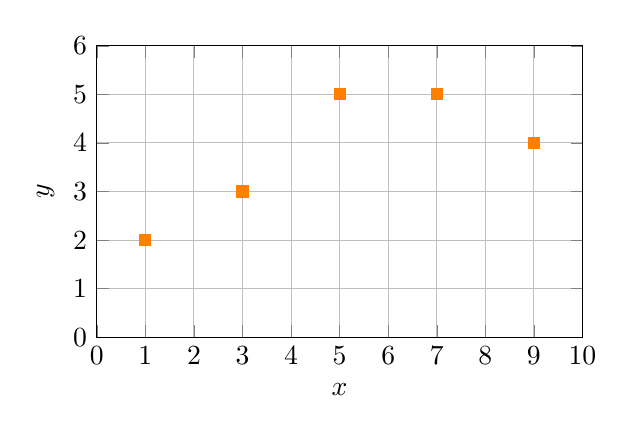
\begin{tikzpicture}
    \begin{axis}[
        scale=0.9, axis equal image,
        xmin=0, xmax=10, xtick={0,...,10},
        ymin=0, ymax=6, ytick={0,...,6},
        samples=50, grid=major, xlabel=$x$, ylabel=$y$]
        \addplot [
            scatter,
            only marks,
            point meta=explicit symbolic,
            scatter/classes={
                a={mark=square*,orange},
                b={mark=triangle*,red}
            },
            nodes near coords*={},
            visualization depends on={\thisrow{myvalue} \as \myvalue},
        ] table [meta=label] {
            x y label myvalue
            1 2 a 1
            3 3 a 1
            5 5 a 1
            7 5 a 1
            9 4 a 1
        };
    \end{axis}
    \end{tikzpicture}
    \end{center}
    \begin{soln} Piecewise linear with all components parallel to the x-axis, passing through the points, i.e., line segment from $x\in [0,2]$ at $y=2$, then $x\in [2,4]$ at $y=3$ etc... \end{soln}
    \begin{qauthor} Matt (Solution by Henry) \end{qauthor}

\part[2] Draw the function that a decision tree regression model with features of the form $x < c$ would learn on the dataset below.

    \begin{center}
    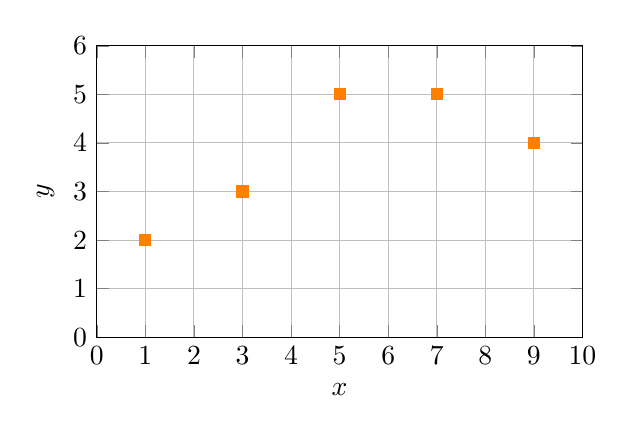
\begin{tikzpicture}
    \begin{axis}[
        scale=0.9, axis equal image,
        xmin=0, xmax=10, xtick={0,...,10},
        ymin=0, ymax=6, ytick={0,...,6},
        samples=50, grid=major, xlabel=$x$, ylabel=$y$]
        \addplot [
            scatter,
            only marks,
            point meta=explicit symbolic,
            scatter/classes={
                a={mark=square*,orange},
                b={mark=triangle*,red}
            },
            nodes near coords*={},
            visualization depends on={\thisrow{myvalue} \as \myvalue},
        ] table [meta=label] {
            x y label myvalue
            1 2 a 1
            3 3 a 1
            5 5 a 1
            7 5 a 1
            9 4 a 1
        };
    \end{axis}
    \end{tikzpicture}
    \end{center}
    \begin{soln} Very similar to part (b) except the line segments to do not need to end exactly at the midpoints between the orange squares; should still be piecewise linear with components parallel to the x-axis. \end{soln}
    \begin{qauthor} Matt (Solution by Henry) \end{qauthor}

\end{parts}
    
\clearpage

\question[1] \textbf{Select one:} How many parameters does a linear regression model on 2-dimensional inputs have?
\begin{checkboxes}
    \choice $0$
    \choice $1$
    \choice $2$ 
    \choice $3$ 
\end{checkboxes}
\begin{soln}
    3
\end{soln}
\begin{qauthor}
   Henry
\end{qauthor}
    
\question We wish to learn a linear regression model on data $\Dc = \{ (\vec{x}^{(i)}, y^{(i)}) \}_{i=1}^N$ For this question, define the pointwise exponential squared error as
\[
    J^{(i)}\Big(\vec{\theta}\Big)=\textrm{exp}\bigg(\frac{1}{2}\Big(y^{(i)} - \vec{\theta}^T\vec{x}^{(i)}\Big)^2\bigg)
\]
Suppose we are interested in minimizing the \emph{geometric} mean of the exponential squared errors over our training data. Recall that the geometric mean of a set of values \\ $\{x^{(1)}, \ldots, x^{(n)}\}$ is the $n^{\textrm{th}}$ root of their product. Thus, our objective in this setting is
\[
    J\Big(\vec{\theta}\Big)=\bigg(\prod_{i=1}^N J^{(i)}(\vec{\theta})\bigg)^{\frac{1}{N}}
\]

\begin{parts}
    \part[2] What is the partial derivative of $J^{(i)}\Big(\vec{\theta}\Big)$ with respect to the $j^{\textrm{th}}$ parameter, $\theta_j$?
    \begin{tcolorbox}[fit,height=3cm, width=15cm, blank, borderline={1pt}{-2pt}]
        %solution
    \end{tcolorbox}
    \begin{soln}
        \begin{align}
            \frac{\partial J^{(i)}}{\partial \theta_j} &= \frac{\partial}{\partial \theta_j}\Bigg(\textrm{exp}\bigg(\frac{1}{2}\Big(y^{(i)} - \vec{\theta}^T\vec{x}^{(i)}\Big)^2\bigg)\Bigg) \nonumber \\ 
            &= \textrm{exp}\bigg(\frac{1}{2}\Big(y^{(i)} - \vec{\theta}^T\vec{x}^{(i)}\Big)^2\bigg)\frac{\partial}{\partial \theta_j}\frac{1}{2}\Big(y^{(i)} - \vec{\theta}^T\vec{x}^{(i)}\Big)^2 \nonumber \\
            &= \textrm{exp}\bigg(\frac{1}{2}\Big(y^{(i)} - \vec{\theta}^T\vec{x}^{(i)}\Big)^2\bigg)\Big(y^{(i)} - \vec{\theta}^T\vec{x}^{(i)}\Big)\Big(-x^{(i)}_j\Big) \nonumber
        \end{align}
    \end{soln}
    \begin{qauthor}
       Henry
    \end{qauthor}
    
    \part[2] What is the gradient of $J^{(i)}\Big(\vec{\theta}\Big)$ with respect to the vector $\vec{\theta}$?
    \begin{tcolorbox}[fit,height=3cm, width=15cm, blank, borderline={1pt}{-2pt}]
        %solution
    \end{tcolorbox}
    \begin{soln}
        \begin{align}
            \frac{\partial J^{(i)}}{\partial \vec{\theta}} &= \frac{\partial}{\partial \vec{\theta}}\Bigg(\textrm{exp}\bigg(\frac{1}{2}\Big(y^{(i)} - \vec{\theta}^T\vec{x}^{(i)}\Big)^2\bigg)\Bigg) \nonumber \\ 
            &= \textrm{exp}\bigg(\frac{1}{2}\Big(y^{(i)} - \vec{\theta}^T\vec{x}^{(i)}\Big)^2\bigg)\frac{\partial}{\partial \vec{\theta}}\frac{1}{2}\Big(y^{(i)} - \vec{\theta}^T\vec{x}^{(i)}\Big)^2 \nonumber \\
            &= \textrm{exp}\bigg(\frac{1}{2}\Big(y^{(i)} - \vec{\theta}^T\vec{x}^{(i)}\Big)^2\bigg)\Big(y^{(i)} - \vec{\theta}^T\vec{x}^{(i)}\Big)\Big(-\vec{x}^{(i)}\Big) \nonumber
        \end{align}
    \end{soln}
    \begin{qauthor}
       Henry
    \end{qauthor}
    
    % \part[1] \textbf{Select one:} Using the design matrix, $X$, and the vector of outputs, $\vec{y}$, which of the following is the gradient of $J\Big(\vec{\theta}\Big)$ with respect to the vector $\vec{\theta}$? 
    % \begin{checkboxes}
    %    \choice $\textrm{exp}\bigg(\frac{1}{2N}\Big(X\vec{\theta} - \vec{y}\Big)^T\Big(X\vec{\theta} - \vec{y}\Big)\bigg)\frac{1}{N}\big(X^TX\vec{\theta}-X^T\vec{y}\big)$ 
    %    \choice $\textrm{exp}\bigg(\frac{1}{2N}\Big(X\vec{\theta} - \vec{y}\Big)^T\Big(X\vec{\theta} - \vec{y}\Big)\bigg)\frac{1}{2N}\Big(X\vec{\theta} - \vec{y}\Big)^T\Big(X\vec{\theta} - \vec{y}\Big)$
    %    \choice $\textrm{exp}\bigg(\frac{1}{N}\big(X^TX\vec{\theta}-X^T\vec{y}\big)\bigg)\frac{1}{2N}\Big(X\vec{\theta} - \vec{y}\Big)^T\Big(X\vec{\theta} - \vec{y}\Big)$
    %    \choice $\textrm{exp}\bigg(\frac{1}{N}\big(X^TX\vec{\theta}-X^T\vec{y}\big)\bigg)\frac{1}{N}\big(X^TX\vec{\theta}-X^T\vec{y}\big)$ 
    % \end{checkboxes}
    % \begin{soln}
    %    Making use of some exponential identities, we can rewrite $J\Big(\vec{\theta}\Big)$ as 
    %    \begin{align}
    %J^{(i)}(\vec{\theta})\bigg)^{\frac{1}{N}} \nonumber \\
    %        &= \Bigg(\prod_{i=1}^N \textrm{exp}\bigg(\frac{1}{2}\Big(y^{(i)} - \vec{\theta}^T\vec{x}^{(i)}\Big)^2\bigg)\Bigg)^{\frac{1}{N}} \nonumber \\
    %        &= \Bigg(\textrm{exp}\bigg(\sum_{i=1}^N \frac{1}{2}\Big(y^{(i)} - \vec{\theta}^T\vec{x}^{(i)}\Big)^2\bigg)\Bigg)^{\frac{1}{N}} \nonumber \\
    %        &= \textrm{exp}\bigg(\frac{1}{N}\sum_{i=1}^N \frac{1}{2}\Big(y^{(i)} - \vec{\theta}^T\vec{x}^{(i)}\Big)^2\bigg) \nonumber
    %    \end{align}
    %    which we can recognize as just the mean squared error exponentiated. Thus, the gradient of $J\Big(\vec{\theta}\Big)$ with respect to the vector $\vec{\theta}$ is
    %    \begin{align}
    %        \frac{\partial J}{\partial \vec{\theta}} &= \frac{\partial}{\partial \vec{\theta}}\textrm{exp}\bigg(\frac{1}{N}\sum_{i=1}^N \frac{1}{2}\Big(y^{(i)} - \vec{\theta}^T\vec{x}^{(i)}\Big)^2\bigg) \nonumber \\ 
    %        &= \textrm{exp}\bigg(\frac{1}{N}\sum_{i=1}^N \frac{1}{2}\Big(y^{(i)} - \vec{\theta}^T\vec{x}^{(i)}\Big)^2\bigg)\frac{1}{N} \frac{\partial}{\partial \vec{\theta}}\sum_{i=1}^N \frac{1}{2}\Big(y^{(i)} - \vec{\theta}^T\vec{x}^{(i)}\Big)^2 \nonumber \\
    %        &= \textrm{exp}\bigg(\frac{1}{2N}\Big(X\vec{\theta} - \vec{y}\Big)^T\Big(X\vec{\theta} - \vec{y}\Big)\bigg)\frac{1}{N}\big(X^TX\vec{\theta}-X^T\vec{y}\big) \nonumber
    %    \end{align}
    % \end{soln}
    % \begin{qauthor}
    %    Henry
    % \end{qauthor}
    
    Using the design matrix, $X$, and the vector of outputs, $\vec{y}$, we can express the gradient of $J\Big(\vec{\theta}\Big)$ with respect to the vector $\vec{\theta}$ as
    \[
        \nabla_{\vec{\theta}} J\Big(\vec{\theta}\Big) = \textrm{exp}\bigg(\frac{1}{2N}\Big(X\vec{\theta} - \vec{y}\Big)^T\Big(X\vec{\theta} - \vec{y}\Big)\bigg)\frac{1}{N}\big(X^TX\vec{\theta}-X^T\vec{y}\big)
    \]
    
    % \part[2] What is the closed-form solution for the optimal parameter vector $\vec{\theta}^*=\textrm{argmin }J\Big(\vec{\theta}\Big)$?
    % \begin{tcolorbox}[fit,height=3cm, width=15cm, blank, borderline={1pt}{-2pt}]
        % solution
    % \end{tcolorbox}
    
    \part[2] \textbf{True or False:} The optimal parameter vector in this setting is $\vec{\theta}^* = \big(X^TX)^{-1}X^T\vec{y}$, the same as the optimal parameter vector for minimizing the mean squared error.
    \begin{checkboxes}
        \choice True 
        \choice False
    \end{checkboxes}
    \begin{soln}
        True; because $\exp(x) > 0$ $\forall$ $x$, when we set the gradient above equal to zero, we can divide both sides by the exponential term and recover the OLS solution: 
        \[
            \vec{\theta}^*=\big(X^TX)^{-1}X^T\vec{y}
        \]
    \end{soln}
    \begin{qauthor}
       Henry
    \end{qauthor}
\end{parts}


\end{questions}